\documentclass[hidelinks=true]{article}
\usepackage[utf8]{inputenc}
\usepackage{graphicx}
\usepackage{verbatim}
\renewcommand{\baselinestretch}{1.5}
\usepackage{indentfirst}
\usepackage[margin=1.2in]{geometry}
\usepackage{placeins}
\usepackage{array}
\usepackage{hyperref}

\begin{document}

\begin{center}
\begin{figure}[h]
\hfill
\includegraphics[]{logo.png}\hspace*{\fill}
\end{figure}
\Large{\textbf{J.S.S. Mahavidyapeetha's}}\\
\LARGE{\textbf{SRI JAYACHAMARAJENDRA COLLEGE OF ENGINEERING, MYSURU}}

\vspace{50pt}
\textbf{Topic : Simulation of Airline Reservation System.}\\ \normalsize (Project work as a part of partial fulfillment of course of Database Management System)
\end{center}

\vspace{40pt}

\large
\textbf{Project team members :}

Samarth Deyagond 
\vspace*{-5pt}

USN : 4JC14CS087
\vspace*{-5pt}

Email Id: \href{deyagondsamarth@gmail.com}{deyagondsamarth@gmail.com}

Rachana K
\vspace*{-5pt}

USN : 4JC14CS073
\vspace*{-5pt}

Email Id: \href{rachanademilovato@gmail.com}{rachanademilovato@gmail.com}
\vspace{30pt}

\large
\textbf{Guides :}

Prof. Manimala S

Prof. Trisiladevi Nagavi

Prof. G. Madhusudan

Prof. Varsha
\pagebreak

\begin{center}
\LARGE{{\textbf{TABLE OF CONTENTS}}}
\end{center}
\hypersetup{hidelinks}
\tableofcontents

\Large{\textbf{References}}

\Large{\textbf{Appendix A}}

\pagebreak


\section{Abstract}
\large    
This project of \textbf{ReplicaDB} is a airline reservation system that is simulated to a good extent in comparison with the existing systems. Basically, it belongs DBMS domain. We have employed Python-Flask framework for implementation of front-end and middleware and in the back-end, MySQL-server client is used.

The project aims at providing user a website where they can find and book flight tickets and enjoy other facilities provided by various airline companies. Other functionalities like canceling tickets, viewing their ticket history is also implemented. The project aims at creating the user-friendly interface and make sure that the changes are reflected in the database.
\pagebreak
\begin{center}
\topskip0pt
\vspace*{\fill}
\LARGE{\textbf{CHAPTER 1 : INTRODUCTION}}
\vspace*{\fill}
\end{center}





\pagebreak

\section{Introduction}

\large \emph{The economic status of a nation is measured by several parameters and transport sector is one main parameter among all.}
\vspace*{10pt}

The Airline Reservation System project is an implementation of a general Airline
Ticketing website like Orbitz and MakeMyTrip, which helps the customers to search the availability and prices of various airline tickets, along with the different packages available with the reservations. This project also covers various features like online registration of the users, by adding, deleting or modifying the customer details, flights or packages information. In general, this website would be designed to perform like any other airline ticketing website available online. 
\vspace*{10pt}

The website is named as \textbf{ReplicaDB} and is the database to access and book the domestic flights whose cost of service is extremely reasonable.

\subsection{Aim}

To simulate an airline reservation database using which people can find flight schedule and enjoy all sorts of services provided by a particular airline company.

\subsection{Objective}
The main objectives of our project are :
\begin{itemize}
\item {To simulate an airline reservation system.}
\item{Using this people can check for schedule, book their tickets, cancel booked tickets, view ticket history and change their account credentials too.}
\item {To develop an user-friendly front-end using suitable tools like Python-Flask so as to make the above operations easy.}
\end{itemize}
\pagebreak
\subsection{Scope}

The scope of the project is as follows : 
\begin{itemize}
\item {The project gives the provision to book one-way journey ticket to the users.}
\item {The database is exclusively for domestic flights with few destinations.}
\item{The front-end is designed only for the client/user end and not the admin end as linking admin end is not a secure plan because of threats of SQL injections and similar malicious activities.}
\end{itemize}

\pagebreak
\begin{center}
\topskip0pt
\vspace*{\fill}
\LARGE{\textbf{CHAPTER 2 : SYSTEM REQUIREMENTS AND ANALYSIS}}
\vspace*{\fill}
\end{center}

\pagebreak

\section{System Requirements}
\subsection{Software Requirements}
\begin{itemize}
\item {Operating System : Windows 10/ Ubuntu 16.04 or equivalent.}
\item{Software : Sublime Text editor, MySQL server-client, any stable browser.}
\item {Front-end : Python-Flask web framework}
\item {Back-end : MySQL server-client version $5.7$}
\item {Middleware : Python MySQLdb module. }
\end{itemize}


\subsection{Hardware Requirements}
\begin{itemize}
\item Processor : 2.2 GHz
\item RAM : 4 GB
\item Input Device : Standard keyboard and mouse
\item Output Device : Monitors with decent resolution.
\end{itemize}

\subsection{Functional Requirements}
\begin{itemize}
\item {Collection of flight schedule : \\ \small{ The schedule of the flight services from different airline companies is to be collected and populated into the database.}}

\item {Redundancy check: \\ \small{The schedule must be verified for redundancy and clashes in the runway timings.}}
\item {Graphical User Interface : \\ \small{A graphical user interface has been designed to pass the control to the built system and display the results.}}
\end{itemize}

\subsection{Non-Functional requirements}
\begin{itemize}
\item {Usability :  \\ \small{The graphical user interface (GUI)} must be user-friendly.}
\item {Accuracy and perfection : \\ \small{The results of the queried operation must generate the required results and make the expected changes as well; with highest accuracy.}}
\end{itemize}

\subsection{Input Requirements}
\begin{itemize}
\item Input of city names as source and destinations.
\item Input of date of journey and number of seats to be booked.
\end{itemize}

\subsection{Output Requirements}
\begin{itemize}
\item Acknowledgement of proper ticket generation and updation of the database.
\end{itemize}

\pagebreak
\begin{center}
\topskip0pt
\vspace*{\fill}
\LARGE{\textbf{CHAPTER 3 : SYSTEM DESIGN AND ANALYSIS}}
\vspace*{\fill}
\end{center}

\pagebreak
\section{System Design}
\subsection{Database Implementation}
\subsubsection{Tools used}
MySQL server-client was employed for the implementation of the database which has the entities and relations as shown in the ER-diagram in figure 1. MySQL is a fast, easy-to-use RDBMS being used for many small and big businesses. MySQL is developed, marketed, and supported by MySQL AB, which is a Swedish company. MySQL is becoming so popular because of many good reasons:

\begin{itemize}
\item {MySQL is released under an open-source license. So you have nothing to pay to use it.}
\item {MySQL is a very powerful program in its own right. It handles a large subset of the functionality of the most expensive and powerful database packages.}
\item {MySQL uses a standard form of the well-known SQL data language.}
\item{MySQL works on many operating systems and with many languages including PHP, PERL, C, C++, JAVA, etc.}
\item{MySQL works very quickly and works well even with large data sets.}
\item {MySQL is very friendly to PHP, the most appreciated language for web development.}
\item{MySQL supports large databases, up to 50 million rows or more in a table. The default file size limit for a table is 4GB, but you can increase this (if your operating system can handle it) to a theoretical limit of 8 million terabytes (TB).}
\item{MySQL is customizable. The open-source GPL license allows programmers to modify the MySQL software to fit their own specific environments.}
\end{itemize}

\begin{figure}
\includegraphics[width = 1\textwidth, height = 19cm]{schema.png}
\caption{Typical schema Diagram of the proposed database}
\end{figure}
%This is schema diagram section
\begin{figure}
\includegraphics[width = 1\textwidth]{erd.png}
\caption{Typical ER Diagram of the proposed database}
\end{figure}


\pagebreak
\subsubsection{Design and building of database.}
The replicaDB has six entities as shown in the ER diagram which are Airline Company, Airplane, Airport, Booked Tickets, Schedule and Users whose attributes go like this:
\begin{itemize}
\item {Airport : \underline{Airport Code}, Airport Name, City, State, Country}
\item {Airline Company : \underline{Company Id}, Company Name}
\item {Airplane : \underline{Airplane Number}, Seating Capacity, Company Id}
\item{Schedule: \underline{Trip Id}, Airline Id, Airplane Id, Source, Destination, Depart, Arrival, Remaining seats in Economy Class, Remaining seats in Business Class, Remaining seats in First Class, Base Fare}
\item{Booked Tickets : \underline{Ticket Id}, user Id, trip Id, Count, Class, Allotted Seat Numbers}
\end{itemize}

\vspace*{10pt}
The MySQL queries to create the above tables are as follows (in the sequence as above):
\vspace{10pt}
\normalsize
\begin{verbatim}

CREATE airport (airportCode INT PRIMARY KEY AUTO_INCREMENT,
airportName VARCHAR(100) NOT NULL, city VARCHAR(50) NOT NULL,
state VARCHAR(50) NOT NULL, country VARCHAR(50) NOT NULL);

CREATE airlineCompany (companyId INT PRIMARY KEY AUTO_INCREMENT,
companyName VARCHAR(100) NOT NULL);

CREATE airplane (airplaneNumber INT PRIMARY KEY AUTO_INCREMENT,
seatingCapacity INT NOT NULL, companyId INT NOT NULL);

CREATE schedule (tripId INT PRIMARY KEY AUTO_INCREMENT,
airlineId INT NOT NULL, airplaneId INT NOT NULL, source VARCHAR(100) 
NOT NULL, destination VARCHAR(100) NOT NULL,
depart DATE, arrival DATE, economyClass INT NOT NULL,
businessClass INT NOT NULL, fisrtClass INT NOT NULL, 
baseFare INT NOT NULL);

CREATE bookedTickets (ticketId INT PRIMARY KEY AUTO_INCREMENT,
userId INT NOT NULL, tripId INT NOT NULL,count INT NOT NULL,
class VARCHAR(50) NOT NULL, seatNumbers VARCHAR(100));
\end{verbatim}

\small \begin{flushleft}
\begin{itemize}
\item {\large{Airport}}
\vspace{5pt}

 \begin{tabular}{|c| c| c| c| c|} 
 \hline
 Airport Code & Airport Name & City & state & Country \\ [0.5ex] 
 \hline\hline
 1 & ChatrapathiShivaji International Airport & Mumbai & Maharashtra & India \\ 
 \hline
 2 & Kempegowda International Airport & Bengaluru & Karnataka & India \\ [1ex] 
 \hline
\end{tabular}
\end{itemize}
\end{flushleft}

\vspace{20pt}
\begin{flushleft}
\begin{itemize}
\item {\large{Airline Company}}\\
\vspace{5pt}

\begin{tabular}{|c | c|} 
\hline
 CompanyId & CompanyName  \\ [0.5ex] 
 \hline\hline
 11 & AirAsia \\ 
 \hline
 12 & AirIndia \\ [1ex] 
 \hline
\end{tabular}
\end{itemize}
\end{flushleft}

\vspace{20pt}
\begin{flushleft}
\begin{itemize}
\item {\large{Airplane}}\\
\vspace{5pt}

 \begin{tabular}{|c| c| c|} 
 \hline
 Airplane Number & Seating Capacity & CompanyId \\ [0.5ex] 
 \hline\hline
 10 & 100 & 11 \\ 
 \hline
 20 & 100 & 12 \\ [1ex] 
 \hline
\end{tabular}
\end{itemize}
\end{flushleft}

\vspace{20pt}
\begin{flushleft}
\begin{itemize}
\item {\large{Users}}\\
\vspace{5pt}

 \begin{tabular}{|c | c | c | c | } 
 \hline
 Id & Name & Email & Password \\ [0.5ex] 
 \hline\hline
 1 & Ria & rria67@gmail.com & flyingsquirrel \\ 
 \hline
 2 & Ishu & ishuchetty14@yahoo.com & rose\\ [1ex] 
 \hline
 3 & Dummakka & dummakkademilovato@gmail.com & Dummi\\ [1ex] 
 \hline
\end{tabular}
\end{itemize}
\end{flushleft}

\vspace{20pt}
\begin{flushleft}
\begin{itemize}
\item {\large{Schedule}}
\vspace{5pt}

\tiny
 \begin{tabular}{|c |c |c |c |c |c |c |c |c |c |c |} 
 \hline
 TripId & AirlineId & AirplaneId & Source & Destination & Depart & Arrival & Economy &Business & First & Basefare \\ [0.5ex] 
 \hline\hline
 90 & 11 & 10 & Mumbai & Bengaluru & 2016-11-09 & 2016-11-09 & 60 & 15 & 10 & 5000 \\ 
 \hline
 91 & 12 & 20 & Bengaluru & Delhi & 2016-11-09 & 2016-11-09 & 60 & 15 & 15 & 6000 \\ [1ex] 
 \hline
\end{tabular}
\end{itemize}
\end{flushleft}

\vspace{20pt}
\begin{flushleft}
\begin{itemize}
\item {\large{Booked Ticket}}\\
\vspace{5pt}

 \begin{tabular}{|c | c | c | c | c | c |} 
 \hline
 TicketId & UserId & TripId & Count & Class & SeatNumbers\\ [0.5ex] 
 \hline\hline
 111 & Ria & 90 & 3 & Economy & 58 to 60 \\ 
 \hline
 2222 & Ishu & 91 & 1 & Business & 75 \\ [1ex] 
 \hline
\end{tabular}
\end{itemize}
\end{flushleft}

\begin{center}
\vspace{10pt} Typical view of populated tables in the database.
\end{center}

\subsubsection{Normal form description of the designed database}
\large
\textbf{Normalization : }

If a database design is not perfect, it may contain anomalies, which are like a bad dream for any database administrator. Managing a database with anomalies is next to impossible. There are many type of anomalies :
\begin{itemize}
\item \textbf{Update anomalies } - When the data items are scattered and are not linked properly, then strange things may happen. Such a situation is update anomaly.
\item \textbf{Delete anomalies } - A data is deleted and a part of it is remaining undeleted also consuming memory because of unawareness. This leads to Delete Anomalies.
\item \textbf{Insert anomalies } - Trying to insert data in a record that doesn't exist leads to Insert anomalies.
\end{itemize}

Normalization is a method to remove all these anomalies and bring the database to a consistent state. \textbf{\emph{Our Database is in Boyce-Codd Normal Form as per our analysis}}. The justification goes like this - 
\begin{itemize}
\item DB holds First Normal Form because all the attributes are atomic in nature.
\item DB also holds Second Normal Form because every non-primary attribute is fully functionally dependent on the prime attribute in the given table.
\item The Boyce-Codd Normal Form also holds good as for any non-trivial functional dependency X-$>$A, X is a super key.
\end{itemize}

Thus replicaDB is in BCNF.
\pagebreak

\subsection{Front-end Implementation and Connectivity}
\subsubsection{Tools used}


\begin{itemize}
\item \textbf{\large Python-Flask} : \\ \normalsize{Flask is a web application framework written in Python. Armin Ronacher, who leads an international group of Python enthusiasts named Pocco, develops it. Flask is based on Werkzeug WSGI toolkit and Jinja2 template engine. Both are Pocco projects.}
\vspace{10pt}
\item \textbf{\large What is framework ?} \\ \normalsize{Web Application Framework or simply Web Framework represents a collection of libraries and modules that enables a web application developer to write applications without having to bother about low-level details such as protocols, thread management etc.}
\vspace{10pt}
\item \textbf{\large WSGI : } \\ \normalsize{Web Server Gateway Interface (WSGI) has been adopted as a standard for Python web application development. WSGI is a specification for a universal interface between the web server and the web applications.}
\vspace{10pt}
\item \textbf{\large Werkzeug : } \\ \normalsize{It is a WSGI toolkit, which implements requests, response objects, and other utility functions. This enables building a web framework on top of it. The Flask framework uses Werkzeug as one of its bases.}
\vspace{10pt}
\item \textbf{\large Jinja2 : } \\ \normalsize{Jinja2 is a popular templating engine for Python. A web templating system combines a template with a certain data source to render dynamic web pages.}
\end{itemize}

\large
Flask is often referred to as a micro framework. It aims to keep the core of an application simple yet extensible. Flask does not have built-in abstraction layer for database handling, nor does it have form a validation support. Instead, Flask supports the extensions to add such functionality to the application.

\pagebreak
\begin{center}
\topskip0pt
\vspace*{\fill}
\LARGE{\textbf{CHAPTER 4 : SYSTEM IMPLEMENTATION}}
\vspace*{\fill}
\end{center}

\pagebreak
\large
\section{System Implementation}
\subsection{Introduction}

Software design of a system is a process of problem solving and planning for a software
solution. It is the process or art of dening the hardware and software architecture,
components, modules, interfaces, and data for a computer system to satisfy specied
requirements. One could see it as the application of systems theory to computing. The
design of the system is essentially a blueprint, or a plan for a solution for the system.
We consider a system to be set of components with the clear and dened behavior,
which interacts in a xed, dened manner, to produce some behaviour or services to its
environment.
\vspace{10pt}

Our system is used to query the schedule of flights and book tickets, cancel them as well.
\subsection{Overview Of the project : }
\begin{center}
\begin{figure}[ht]
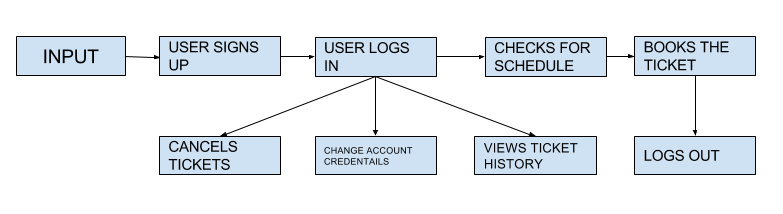
\includegraphics[width=1\textwidth]{process.png}
\caption{Block Diagram Representing Overview of Our Project}
\end{figure}
\end{center}
\pagebreak
\large
\subsection{Implementation Steps}
The entire application is coded in Sublime Text Editor and the tables were populated using the terminal of MySQL server-client interface. We have achieved all the above mentioned objectives in section $1.2$

\begin{itemize}
\item The database was populated with the schedule referring to some Google results for airport details and dates were set randomly by ourselves. Other created tables were kept empty for populating them.
\item The empty table \textbf{users} was populated as and when people signed up.
\item After user signs up automatically is redirected to booking page where input details such as source,destination and travel date is taken from user and verifies
\begin{itemize}
\item if source and destination is same if not then proceeds towards next stage i.e Schedule and information about flight details i.e schedule is displayed to user by fetching details(src,dest,traveldate,companyid,airlineid) from \lq Schedule\rq\  table using \lq select\rq\  command. 
\item if no service provided by any of the airline companies to the specified source and destination.
\end{itemize}
\item  User needs to select the service provided by different airline companies i.e appropriate timing suitable as per their convenience.
\item After choosing the flight, a unique tripid is given and user needs to remember this unique tripid.
\item Using this tripid user will have to input number of seats to be booked along with the type of class, account number and account password for payment.
\item If number of seats entered is available for a particular travel-class, only then booking is confirmed by checking the count of the number of seats that are being booked is not greater than available seats in each travel-class from schedule table.
\item On successful completion of booking stage-2 ticket is confirmed. And these details (Ticketid, userid,tripid, count, class) are inserted into \textbf{bookedTickets} table.
\item The number of seats available in each travel-class (of the flight of that particular tripId) after booking is updated (the number of available seats are reduced to be precise) in \lq schedule\rq\ table using \lq update\rq\ query. 
\item Then \lq cancel ticket\rq\ operation was implemented to delete the tuple from the bookedTickets table. Because canceling a ticket will require the booking history of the particular user, the operation of \emph{fetch booking history} was also implemented. The query is run such that the booked tickets that are dated the cuurent day and the following current day are listed and not the ones whose journey has already taken place.
\item User can check his previous ticket bookings using \lq Ticket History\rq\ option. As the user is still logged in,we can fetch the userid from \lq bookedTickets\rq\ table and fetch tripid from \lq Schedule\rq\ table and display the respective Schedule parameters([tripId,AC,source,destination,depart,arrival,seat,fare) of the previous bookings.


\item User is also provided with option to change email\_id and password in \lq Account Settings\rq\.The new email\_id and new password is updated in \lq Users\rq table.
\item After user is done with booking,he/she can \lq logout\rq\ and the session allocated to that particular user is 
\end{itemize}

\pagebreak
The screen-shots of different windows for specific operation are as follows : 

\begin{figure}[ht]
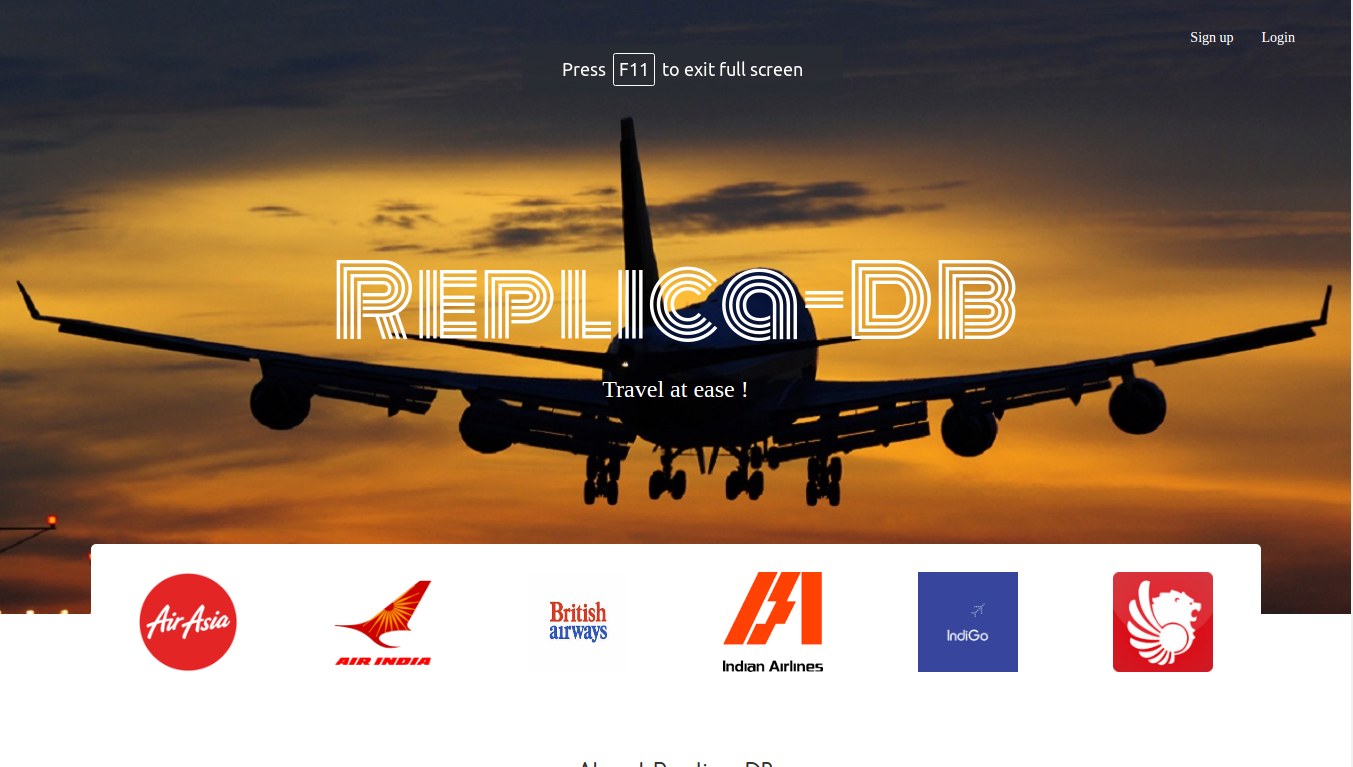
\includegraphics[width=1\textwidth]{home.png}
\caption{The home page of ReplicaDB}
\end{figure}

\begin{figure}[ht]
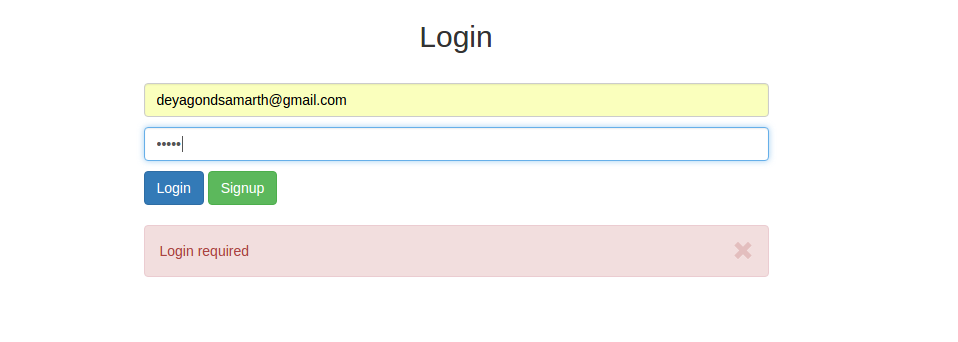
\includegraphics[width=1\textwidth]{login.png}
\caption{The Login page for the user}
\end{figure}

\begin{figure}[ht]
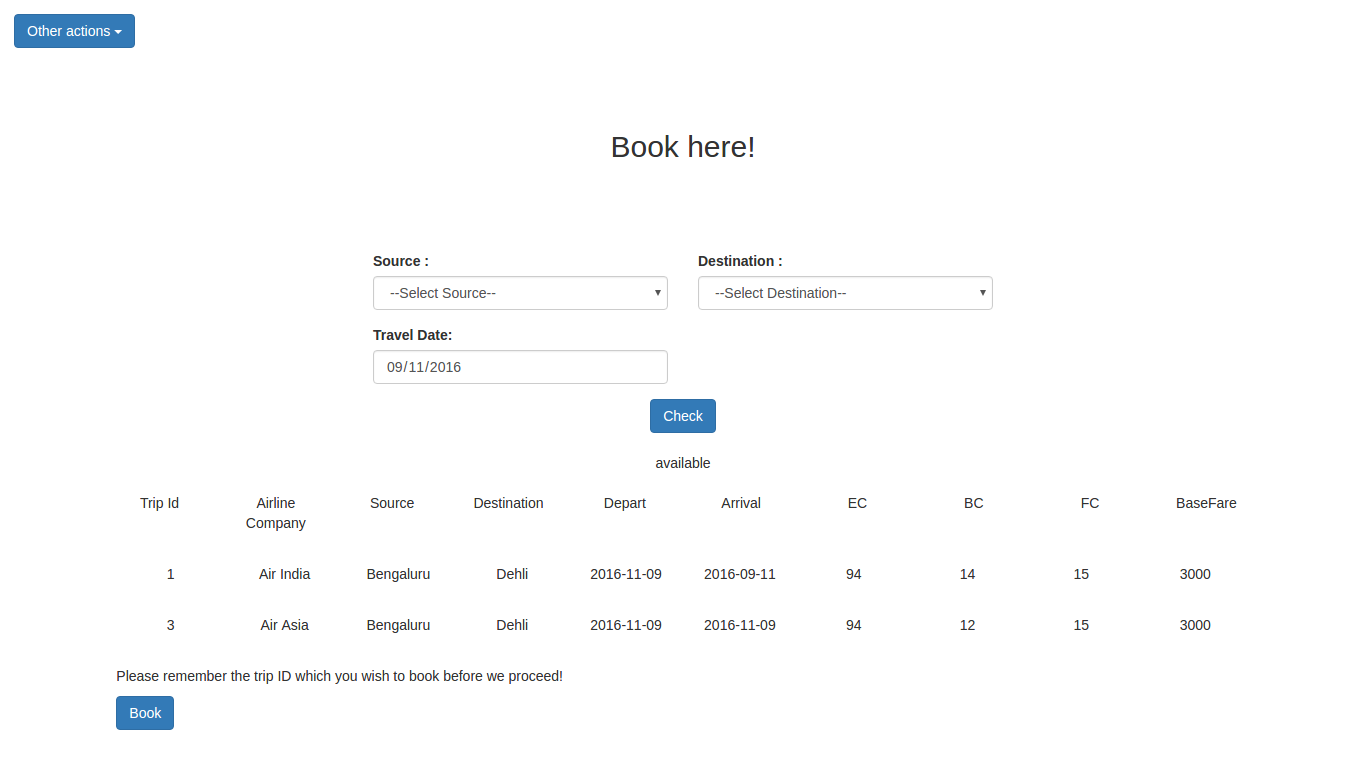
\includegraphics[width=1\textwidth,height=8cm]{booking.png}
\caption{The booking page for the user along with schedule display}
\end{figure}

\begin{figure}[ht]
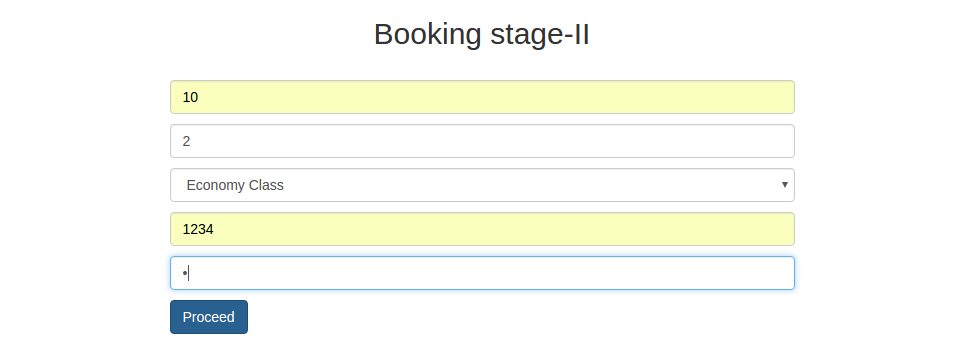
\includegraphics[width=1\textwidth]{booking2.png}
\caption{The stage-2 booking page for the user along with schedule display}
\end{figure}

\begin{figure}[ht]
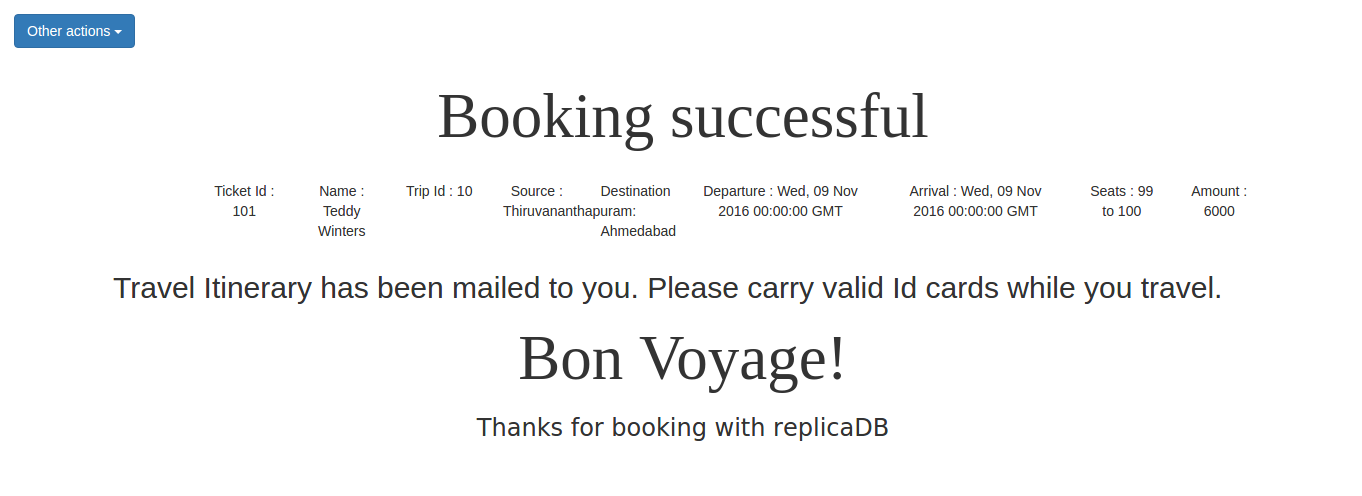
\includegraphics[width=1\textwidth]{ticket.png}
\caption{The generated acknowledgment and travel itinerary }
\end{figure}

\begin{figure}[ht]
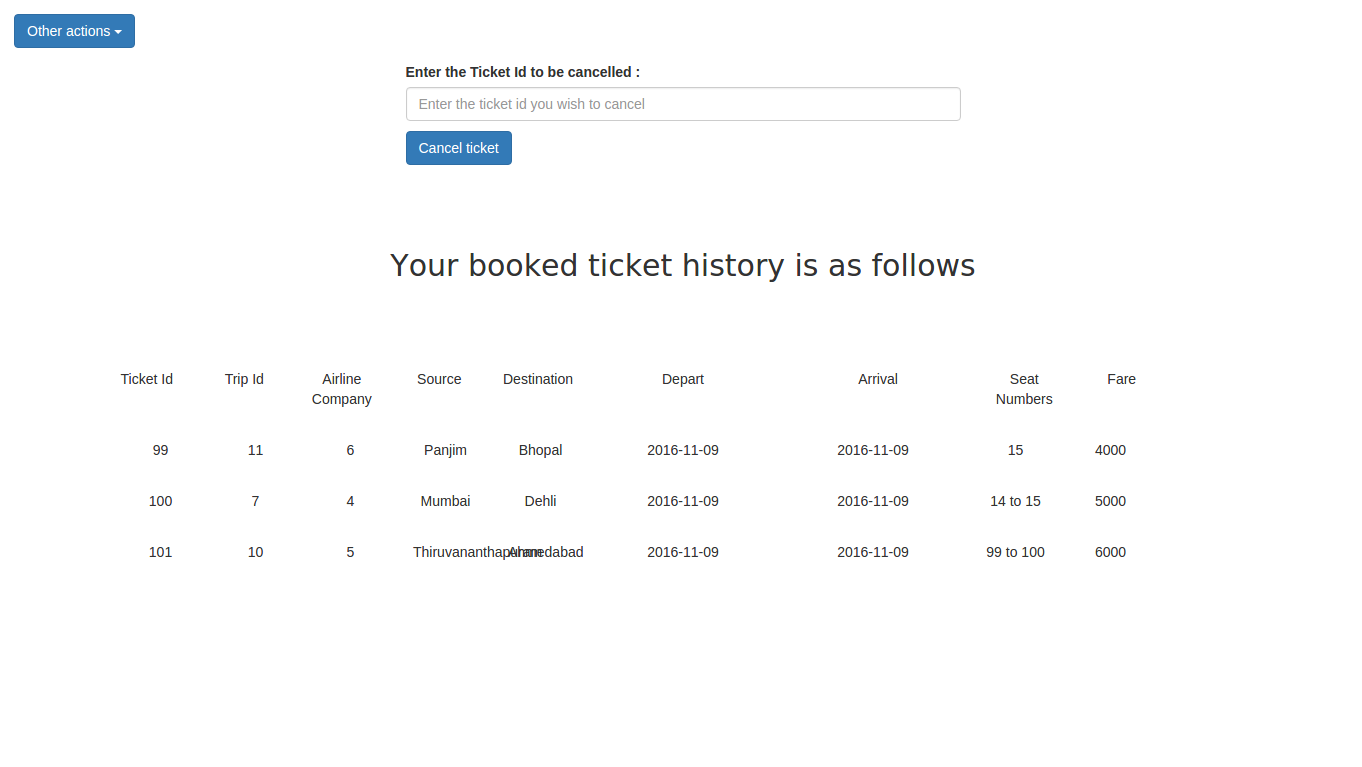
\includegraphics[width=1\textwidth]{cancel.png}
\caption{The interface to cancel the booked tickets along with display of booking history.}
\end{figure}

\begin{figure}[ht]
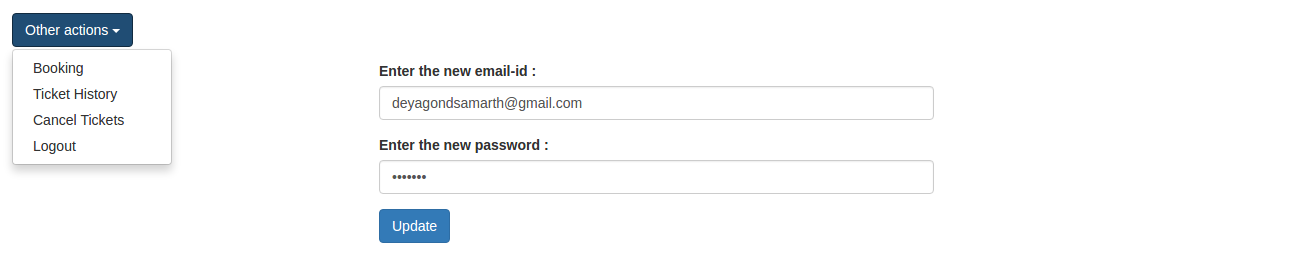
\includegraphics[width=1\textwidth]{update.png}
\caption{A simple interface to update the account credentials. Also navigation drop-down from page to every other page.}
\end{figure}
\FloatBarrier
This way the database so created was connected with the front-end application and it was tested for the reflection of the changes from the front-end onto the database.
\pagebreak
\begin{center}
\topskip0pt
\vspace*{\fill}
\LARGE{\textbf{CHAPTER 5 : SYSTEM TESTING AND CRITICAL ANALYSIS OF RESULTS}}
\vspace*{\fill}
\end{center}
\pagebreak
\section{System Testing and Critical Analysis of results}
\subsection{Uniting testing and result analysis}
Incremental unit testing involves the design of test cases that validate integral program
logic is working properly, and the program input produces valid output.
\vspace{15pt}

\begin{center}
\begin{tabular}{|m{1cm}|m{3cm}|m{3cm}|m{2cm}|m{2cm}|m{2cm}|}
\hline
\centering 
Serial no & \centering Test Case &\centering Description &\centering Expected result &\centering Actual result & Remark \\ \hline
\centering 1 & \centering Populating database & \centering  Checks for INSERT queries & \centering successful insertion & \centering insertion successful & \begin{center}PASS\end{center} \\ \hline
\centering 2 & \centering Updating database & \centering Checks for UPDATE queries and constraint handling & \centering successful update & updation successful &\begin{center}PASS\end{center}\\ \hline
\centering 3 & \centering Deletion of tuples & \centering Checks the DELETE queries & \centering successful deletion & \centering Deletion successful &\begin{center}PASS\end{center}\\ \hline
\end{tabular}
\end{center}
\begin{figure}[ht]
\caption{Unit testing result}
\end{figure}

\subsection{Integration testing}
After the above tests were successfully carried out, the integration testing was conducted where the database (the back-end) was connected to the front-end application which was developed using Python-Flask frame work. It was checked for the same operations which were verified in unit testing with the only change that Python MySQLdb module was used as the middle ware. The functioning of the front-end was pretty good and every expected result was observed. \textbf{\emph{So, integration testing as a whole was given the remark as PASS.}}

\pagebreak
\begin{center}
\topskip0pt
\vspace*{\fill}
\LARGE{\textbf{CHAPTER 6 : CONCLUSION AND FUTURE WORK}}
\vspace*{\fill}
\pagebreak
\end{center}

\section{Conclusion and Future Work}
\subsection{Project conclusion}
The main aim of this project ReplicaDB was to simulate the airline reservation system similar to existing systems like MakeMyTrip or Orbitz. 
However, in future we are looking forward to have the following enhancements :

\begin{itemize}
\item Implementation of package booking including return tickets or round-trip booking concept.
\item To suggest the schedule as per the rating of the passengers who have traveled in a particular airline company's flight. (\emph{For this; to implement, we need lots of dataset to have the recommender system ready using machine learning algorithms}). To accomplish this,we need to run this system for some period of time which is actually decided by the extent of usage of the system by people.
\end{itemize}

\subsection{Write up on personal satisfaction}
With this project we were able to :
\begin{itemize}
\item Design and implement database.
\item Analyze them for their normal forms.
\item Draw proper ER diagram and Schema diagrams.
\item Explore new front-end development tools like Python-Flask.
\item Felt apparently as if we developed a small scale software application.
\end{itemize}
And we have mention to that we got good guidance and support from all the lab in-charge faculties.

\pagebreak
\LARGE{\textbf{References}}
\begin{itemize}
\Large
\item Python Flask documentation - 
\url{http://flask.pocoo.org/docs/0.11/}
\item MySQL documentation - \url{https://help.ubuntu.com/lts/serverguide/mysql.html}
\item MySQLdb beginner's documentation -\url{https://wiki.python.org/moin/BeginnersGuide}
\item Google searches for details of airports in India.
\end{itemize}

\vspace{80pt}
\LARGE{\textbf{Appendix A}}


\normalsize
\listoffigures
\end{document}

